\documentclass[aip,apl,reprint]{revtex4-1}
\usepackage{graphicx}

\begin{document}
%グラフの解像度が荒いのでdev.copy2eps(file="ファイル名.eps")などを用いてRのグラフをepsなどで保存する

\title{Current pulse switching of gray and white tin} 
\author{Nobuyoshi Hiramatsu}
\affiliation{Department of Applied Physics, The University of Tokyo, Tokyo 113-8656, Japan.}
\author{Hiroshi Oike}
\affiliation{Department of Applied Physics, The University of Tokyo, Tokyo 113-8656, Japan.}
\author{Fumitaka Kagawa}
\email[]{kagawa@ap.t.u-tokyo.ac.jp}
\affiliation{Department of Applied Physics, The University of Tokyo, Tokyo 113-8656, Japan.}
\affiliation{RIKEN Center for Emergent Matter Science, Wako 351-0198, Japan.}

\begin{abstract}
White tin exhibits superconductivity with critical temperature 3.7K while gray tin is semiconducting with the band gap $E_g=0.018eV$.
We demonstrated the reversible transformation between semiconductor-tin (gray tin) and metallic superconductor-tin (white-tin) by applying current pulses.
\end{abstract}
%\pacs{}% insert suggested PACS numbers in braces on next line

\maketitle 
\section{Introduction}

\begin{figure}[!h]
    \begin{center}
   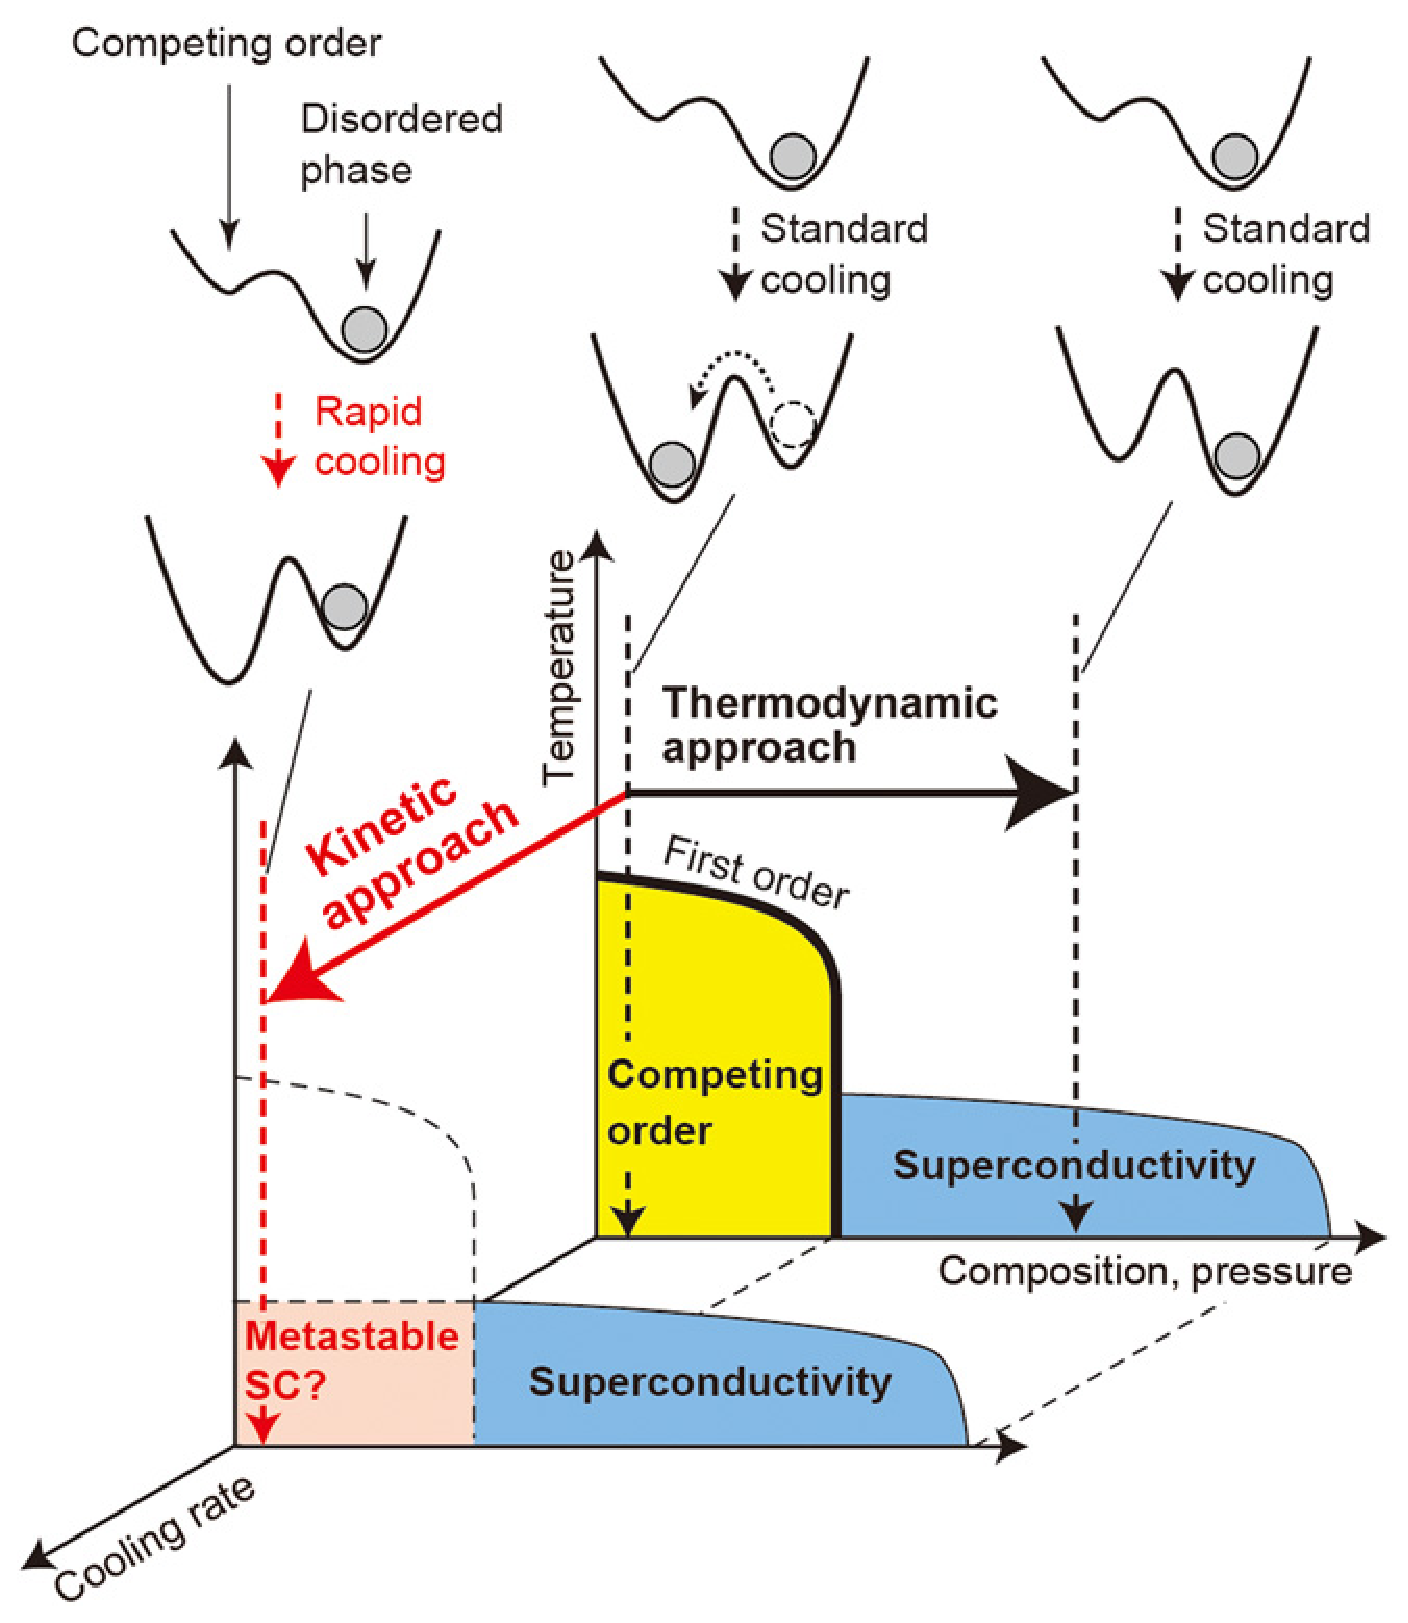
\includegraphics[width=0.9\hsize]{kinetic_approach.eps}
  \end{center}
  \caption{some schematics is needed}
  \label{fig:kinetic_approach.eps}
\end{figure}


\section{method}
\subsection{Sample preparation}
Metallic Sn-Ge alloy was converted to semiconductor in a freezer.
Pure Ge-drops (Furuuchi chemical GEM-33001A) were grind, and mixed with pure Sn-drops (Furuuchi chemical SNM-67027A) in a mass ratio1:99 in a quartz tube. The tube was evacuated and heated up to 1050$^\circ$C and cooled slowly in 48 hours in a electric oven. The melted sample were metallic, and we converted to semiconductor phase in a household freezer for a week. 

\subsection{Connections}
Sample was 

\subsection{Resistivity measurement}
The resistivity under slow cooling was measured with the conventional four-probe method. A load resistor of 150 ohms was connected in series with the sample. An AC voltage excitation of 105 Hz with a magnitude corresponding to ? μA was generated at a lock-in amplifier (Stanford Research SR830) and applied to the circuit. Signals from the voltage probes were amplified with a transformer amplifier (Stanford Research SR554) and measured with the lock-in amplifier. The current flowing through the circuit was measured by probing the voltage drop at the load resistor with a multimeter (Keithley 2001).

\subsection{Pulse application}
A rectangular voltage-pulse generated in a source meter (Keithley 2400) was amplified using a precision power amplifier (NF Corporation 4502) by A=100. A load resistor of 5.4 ohms was connected in series with the sample and used to calculate the current flowing through the circuit. The time-varying voltages at the load resistor and the sample voltage-probes were were monitored using a data logger (Measurement Computing DT8824). Thus, we obtained the time profiles of the current and sample resistivity during the pulse application. 

\begin{figure}[!h]
    \begin{center}
   \includegraphics[width=0.9\hsize]{181228_current_resistance.eps}
  \end{center}
  \caption{}
  \label{fig:181228_current_resistance.eps}
\end{figure}

\begin{figure}[!h]
    \begin{center}
   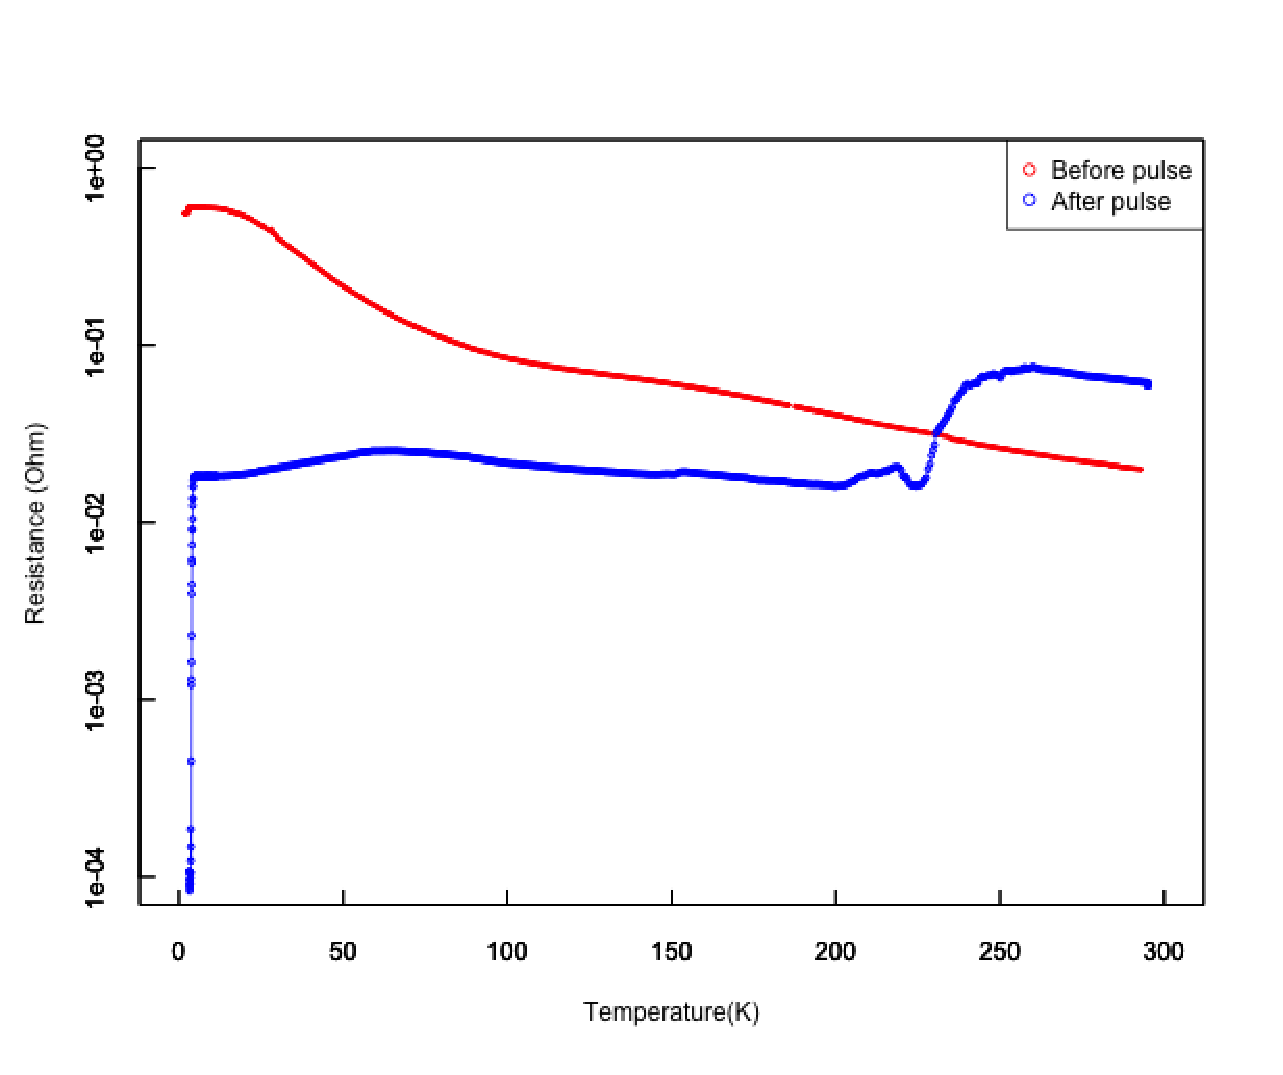
\includegraphics[width=\hsize]{181228_before_after_pulse_log.eps}
  \end{center}
  \caption{a graph that demostrates superconductivity should be inserted in the inset }
  \label{fig:181228_before_after_pulse_log}
\end{figure}

\section{Discussions}
slow\cite{oike}

\section{Conclusion}
We demonstrated the reversible transformation between semiconductor and metallic tin by applying current pulse.

\section{Supplementary materials}
Supplementary material for this article is available at ...

\begin{acknowledgments}
This work was partially supported by the Japan Society for the Promotion of Science KAKENHI (grant nos. 18K13512 and 18H01168).
The authors thank A. Kikkawa for technical support in sample preparation and T. Nakajima for technical support in X-ray crystallography.
\end{acknowledgments}

\bibliography{your-bib-file}

\end{document}